\documentclass[12pt, a4paper]{article}

\usepackage[utf8]{inputenc}
\usepackage{mathtools}
\usepackage{amssymb}
\usepackage{ntheorem}
\usepackage[framemethod=TikZ]{mdframed}
\usepackage{amsmath}
\usepackage[hidelinks]{hyperref}
\usepackage{cleveref}
\usepackage[most]{tcolorbox}
\usepackage{fancyhdr}
\usepackage{lastpage}
\usepackage{geometry}
\usepackage{graphicx}
\usepackage{float} 
\usepackage{subfigure} 
\usepackage{arydshln}
\usepackage{multicol}
\usepackage{url}
\usepackage{setspace}
\usepackage[T1]{fontenc}
\usepackage{mathptmx}

\geometry{a4paper, left=2cm, right=2cm, bottom=2cm, top=2cm}

\definecolor{blue}{rgb}{0,0.45,1.14}
\definecolor{red}{rgb}{0.77,0.12,0.23}
\definecolor{grey}{rgb}{0.49,0.38,0.29}
\definecolor{green}{rgb}{0,0.42,0.24}
\definecolor{SpringGreen}{rgb}{0.95,0.97,0.95}
\definecolor{OliverGreen}{rgb}{0.09,0.34,0.09}
\definecolor{LeftGreen}{rgb}{0.13,0.54,0.13}
\definecolor{orange}{rgb}{2.07,0.69,0.32}

\newtcbtheorem[no counter]{example}{Example}{
  enhanced,
  sharp corners,
  attach boxed title to top left={
    yshifttext=-1mm
  },
  colback=white,
  colframe=blue!25,
  fonttitle=\bfseries,
  coltitle=black,
  boxed title style={
    sharp corners,
    size=small,
    colback=blue!25,
    colframe=blue!25,
  }
}{exm}

\newtcbtheorem[no counter]{theorem}{Theroem}{
  enhanced,
  sharp corners,
  attach boxed title to top left={
    yshifttext=-1mm
  },
  colback=white,
  colframe=grey!25,
  fonttitle=\bfseries,
  coltitle=black,
  boxed title style={
    sharp corners,
    size=small,
    colback=grey!25,
    colframe=grey!25,
  }
}{thm}

\newtcbtheorem[no counter]{proof}{Proof}{
  enhanced,
  sharp corners,
  attach boxed title to top left={
    yshifttext=-1mm
  },
  colback=white,
  colframe=orange!50,
  fonttitle=\bfseries,
  coltitle=black,
  boxed title style={
    sharp corners,
    size=small,
    colback=orange!50,
    colframe=orange!50,
  }
}{proof}

\newtcbtheorem{myclaim}{Definition}{ 
    coltitle=OliverGreen,
    colback=SpringGreen,
    colframe=LeftGreen,
    detach title,
    boxrule=0pt,
    leftrule=2pt,
    attach title to upper,
    sharp corners,
    left=1mm,
}{claim}

\rhead{\thepage}
\linespread{1.15}

\title{\textbf{IB Mathematics Analysis and Approaches HL}\\
Topic 1 Number and Algebra}
\author{Jiuru Lyu}
\date{\today}

\def\Z{{\mathbb{Z}}}
\def\R{{\mathbb{R}}}
\def\C{{\mathbb{C}}}
\def\Q{{\mathbb{Q}}}
\def\E{{\mathbb{E}}}
\def\d{{\mathrm{d}}}
\def\i{{\mathrm{i}}}
\def\RE{{\mathrm{Re}}}
\def\IM{{\mathrm{Im}}}
\def\Arg{{\mathrm{Arg}}}
\def\cis{\mathrm{cis}}

\begin{document}

\maketitle
\tableofcontents

\newpage

\section{Sequences and Series}
\begin{enumerate}
\item Terms: $u_1,\ u_2,\ u_3...$\\Position: $n$\\Sum: $S$
\item \textbf{\color{red}{Arithmetic Sequence}}/Arithmetic Progession (AP): 
  \begin{itemize}
    \item Recursive formula: {\color{red}{$u_{n+1}=u_n+d$}}, $d$ is the common difference.
    \item Explicit formula: {\color{red}{$u_n=u_1+d(n-1)$}}
    \item Summation: \color{red}{$S_n=\frac{1}{2}[2u_1+d(n-1)]$}
      \begin{proof}{1.1.1}{}
        Let $u_1,\ u_2,\ u_3,\ ...,\ u_n$ be an arithmetic sequence with $d$ as common difference. \\
        Then, $S_n=u_1+u_2+u_3+...+u_n=u_1+(u_1+d)+(u_1+2d)+...+(u_1+(n-1)d)$\\
        Also, $S_n=[u_1+(n-1)d]+...+(u_1+d)+u_1.$\\
        Add two expressions together: 
        $$2S_n=[2u_1+(n-1)d]n$$
        $$\therefore S_n=\frac{n}{2}[2u_1+(n-1)d].$$ 
      \end{proof}
  \end{itemize}
\item {\textbf{\color{red}{Geometric Sequence}}}
  \begin{itemize}
    \item Recursive formula: {\color{red}{$u_{n+1}=r \cdot u_n$}}, $r$ is the common ratio.
    \item Explicit formula: {\color{red}{$u_{n}=u_1 \cdot r^{n-1}$}}
    \item $$r=\frac{u_2}{u_1}=\frac{u_3}{u_2}=\frac{u_4}{u_3}=...$$
    \item Summation: {\color{red}{$S_n=\frac{u_1(r^n-1)}{r-1}$}}
    \begin{proof}{1.1.2}{}
      Let $u_1,\ u_2,\ u_3,\ ...,\ u_n$ be a geometric sequence with $r$ as common ratio.\\
      $S_n=u_1+u_2+u_3+...+u_n=u_1+(u_1 \cdot r)+(u_1 \cdot r^2)+...+(u_1 \cdot r^{n-1})$\\
      Then, $rS_n=(u_1\cdot r)+(u_1 \cdot r^2)+...+(u_1 \cdot r^n).$\\
      Substract the first expression from the second: 
      $$rS_n-S_n=u_1 \cdot r^n-u_1 \Rightarrow (r-1)S_n=u_1(r^n-1)$$
      $$\therefore S_n=\frac{u_1(r^n-1)}{r-1}$$
    \end{proof}
    \item If $r>1$, the sequence is an exponential growth.\\If $0<r<1$, the sequence has an exponential decay. 
    \item When $r>1$, series approaches $\infty$.\\{\color{red}{When $-1<r<1$, or $\left|r\right|<1$, the series converges: $$S_\infty=\frac{u_1}{1-r}, \left|r\right|<1$$}}
  \end{itemize} 
\end{enumerate}

\section{Exponents and Logarithms}
\begin{enumerate}
  \item {\color{red}{$a^m \cdot a^n=a^{m+n}\\ a^m \div a^n=a^{m-n}\\ (a^m)^n=a^{mn}$}}
  \item {\color{red}{$x^0=1$}} {\color{green}{($x^0=x^{1-1}=\frac{x^1}{x^1}=1$)}}\\ {\color{red}{$x^{-m}=\frac{1}{x^m}$}}\\ {\color{red}{$x^{\frac{1}{n}}=\sqrt[n]{x}$}} {\color{green}{($x^{\frac{m}{n}}=(\sqrt[n]{x})^m$)}}
  \item If $a=b$, then $a^n=b^n$\\ If $m=n$, then $a^m=a^n$\\ {\color{green}{For $a^b=1$: $a=1, b \in \mathbb{R}$; $a \neq 1, b=0$; OR $a=-1, b=2n$}}
  \item When solving exponential equations, convert them to the same base. 
  \item Division Theorem. 
  \begin{theorem}{1.2.1}{}
    If $a^x=b^y$ given $a>0$ and $b>0$, then {\color{red}{$a=b^{\frac{y}{x}}$}}.
    \begin{proof}{1.2.1}{}
      $$a^x=b^y$$
      $$(a^x)^\frac{1}{x}=(b^y)^\frac{1}{x} \Rightarrow a=b^\frac{y}{x}$$
    \end{proof}
  \end{theorem}
  \item $a=b^x \Leftrightarrow x=\log_b{a}$, where $a,b \in \mathbb{R}^+$ and $b \neq 1$.
  \item Logarithmic rules: 
  \begin{itemize}
    \item {\color{red}{$\log_ax+\log_ay=\log_a(xy)$}}
    \begin{proof}{1.2.2}{}
      Let $\log_ax=p,\ \log_ay=q.\ \Rightarrow a^p=x, a^q=y.$\\
      Then, $x \cdot y=a^p \cdot a^q=a^{p+q}.$
      $$\therefore \log_a(xy)=p+q=\log_ax+\log_ay.$$
    \end{proof}
    \item {\color{red}{$\log_ax-\log_ay=\log_a\left(\frac{x}{y}\right)$}}
    \begin{proof}{1.2.3}{}
      Let $\log_ax=p,\ \log_ay=q.\ \Rightarrow a^p=x, a^q=y.$\\
      Then, $\frac{x}{y}=\frac{a^p}{a^q}=a^{p-q}.$
      $$\therefore \log_a\left(\frac{x}{y}\right)=p-q=\log_ax-\log_ay.$$
    \end{proof}
    \item {\color{red}{$\log_ax^n=n\log_ax$}} 
    \item {\color{red}{$\log_a1=0$}}
    \item {\color{red}{$\log_aa=1$}}
    \item {\color{red}{$-\log_ax=\log_a\frac{1}{x}$}}
    \item {\color{red}{$\log_ax=\frac{\log_bx}{\log_b{a}}$}}
    \item {\color{red}{$s\log_ab=\frac{1}{\log_b{a}}$}}
  \end{itemize}  
\end{enumerate}

\section{Proof}
\begin{enumerate}
  \item Direct proof:
  \begin{example}{1.3.1}{}
    \textbf{Show that the sum of two even numbers is always even.}\\
    \noindent\rule[0.1pt]{\textwidth}{1pt}
    Let $m$ and $n$ be two even positive integers. \\
    $m=2p, n=2q$, where $p$ and $q \in \mathbb{Z}^+$. \\
    Then, $m+n=2p+2q=2(p+q)$, which is an even number. 
  \end{example}
  \begin{example}{1.3.2}{}
    \textbf{Show that $\left(x+\frac{a}{2}\right)^2-\left(\frac{a}{2}\right)^2 \equiv x^2+ax$.}\\
    \noindent\rule[0.1pt]{\textwidth}{1pt}
    $$\text{LHS}=x^2+\frac{a^4}{4}+ax-\frac{a^4}{4}=x^2+ax=\text{RHS}.$$
  \end{example}
  {\color{green}{Equations "$=$": only true from some values.\\Identities "$\equiv$": true for all values.}}
  \begin{example}{1.3.3 Question}{}
    \textbf{Prove that if the sum of the digits of a four-digit number is divisible by $3$, then the four-digit number is also divisible by $3$.}
  \end{example}
  \begin{example}{1.3.3 Answer}{}
    Let $n$ be a 4-digit number: $n=1000a+100b+10c+d$, where $0\leq a,b,c,d\leq 9$, and $a\neq 0$.\\
    It is given that $a+b+c+d=3k, k \in \mathbb{Z}$:
    $$\begin{aligned}
        n&=1000a+100b+10c+d+3k-a-b-c-d\\
        &=999a+99b+9c+3k\\
        &=3(333a+33b+3c+k)
      \end{aligned}$$
    Since $(333a+33b+3c+k)\in \mathbb{Z}$, it implies that $n$ is divisible by 3. 
  \end{example}
  \item Proof by Contradiction: 
  \begin{example}{1.3.4}{}
    \textbf{Prove the statement: If the integer $n$ is odd, then $n^2$ is also odd.}\\
    \noindent\rule[0.25\baselineskip]{\textwidth}{1pt} 
    Let, if possible, $n^2$ is even and $n$ is odd. \\
    Then, $n^2=2k,\ k\in \mathbb{Z} \Rightarrow n\times n=2k$, which indicates the product of two odd number is even, and which is not true. \\
    Hence, there is a contradiction.\\
    $\therefore$ Our assumption is wrong, and thus given that $n$ is odd, $n^2$ is also odd. 
  \end{example}
  \begin{example}{1.3.5}{}
    \textbf{Show that $\sqrt{2}$ is irrational.}\\
    \noindent\rule[0.25\baselineskip]{\textwidth}{1pt} 
    Let us assume, if possible, taht $\sqrt{2}$ is rational: \\
    $\sqrt{2}=\frac{p}{q}$, where $p,q\in \mathbb{Z}$, and $p$, $q$ have no common factors, $q\neq 0$. \\
    $\therefore 2=\frac{p^2}{q^2} \Rightarrow p^2=2q^2 \text{\ \ \ \ \ \ (1).}$\\
    $\therefore p^2$ is even, and thus $p$ is also even. \\
    As $p$ is an even number, we can write: $p=2k, k\in \mathbb{Z}. \Rightarrow \therefore p^2=(2k)^2=4k^2 \text{\ \ \ \ \ \ (2)}.$\\
    From (1) and (2): $4k^2=2q^2 \Rightarrow q^2=2k^2 \Rightarrow q^2$ is even, and thus $q$ is also an even number.\\
    But since $p$ and $q$ have no common factors, they cannot have "2" as a common factor. Hence, we have arrived at a contradiction. \\
    $\therefore$ Our assumption is incorrect, and $\sqrt(2)$ is irrational.
  \end{example}
  \begin{myclaim}{ }{}
    A number is \textbf{\color{red}{rational}} if it can be written as $\frac{p}{q}$, where $p,q\in \mathbb{Z}$, and $q \neq 0$.
  \end{myclaim}
  \begin{example}{1.3.6 Question}{}
    \textbf{Prove that there is no $x\in \mathbb{R}$ such that $\frac{1}{x-2}=1-x$}
  \end{example}
  \begin{example}{1.3.6 Answer}{}
    Assume there is a real number $x$ such that $\frac{1}{x-2}=1-x$. \\
    $\therefore (1-x)(x-2)=1 \Rightarrow x^2-3x+3=0$\\
    Solving the equation, we get $x=\frac{3\pm \sqrt{9-12}}{2}$, which $\notin \mathbb{R}$\\
    $\therefore$ We arrived at a contradiction, and our assumption is incorrect. There is no $x\in \mathbb{R}$ such that $\frac{1}{x-2}=1-x$
  \end{example}
  \item Proof by Mathematical Induction
  \begin{myclaim}{ }{}
    \textbf{\color{red}{Principle of Mathematical Induction (PMI)}}: \\Suppose $P_n$ is a proposition which is defined for every integer $n \geq a,\ a \in \mathbb{Z}$. If $P_a$ is true, and if $P_{k+1}$ is true whenever $P_k$ is true, then $P_n$ is true $\forall n \geq a$.
  \end{myclaim}
  \begin{example}{1.3.7}{}
    \textbf{Prove that $4^n+2$ is divisible by $3$ for $n \in \mathbb{Z},\ n\geq 0$, by using PMI.}\\
    \noindent\rule[0.25\baselineskip]{\textwidth}{1pt} 
    For $n=0$, $\text{LHS}=4^0+2=1+2=3$, which is divisible by 3. \\
    $\therefore P_0$ {\color{green}{(OR denoted as $P(0)$)}} is true. \\
    Assume that $P_k$ is true: i.e., $4^k+2\text{ is divisible by }3$. $\Rightarrow 4^k+2=3A,\ A \in \mathbb{Z}^+ \Rightarrow 4^k=3A-2.$\\
    Consider $P_{k+1}$: 
    $$\begin{aligned}4^{k+1}+2&=4^k\cdot 4^1+2\\
      &=(3A-2)\cdot 4+2\\
      &=12A-6\\
      &=3(4A-2).
    \end{aligned}$$
    $\therefore 4A-2$ is an integer as $A \in \mathbb{Z}^+,\ 4^{k+1}+2$ is divisible by 3 whenever $4^k+2$ is divisible by 3. \\
    Since $P_0$ is true, and $P_{k+1}$ is true whenever $P{k}$ is true, $P_n$ is ture $\forall n \in \mathbb{Z},\ n \geq 0$.
  \end{example}
  \begin{example}{1.3.8}{}
    \textbf{A sequence is defined by $u_{n+1}=2u_n+1\ \forall n \in \mathbb{Z}^+$. Prove that $u_n=2^n-1$.}\\
    \noindent\rule[0.25\baselineskip]{\textwidth}{1pt} 
    For $n=1,\ u_1=2^1-1=1\Rightarrow \therefore P_1$ is ture.\\
    Let $P_k$ be true: $u_k=2^k-1$ for some $k\in\mathbb{Z}^+$.\\
    Consider $P_{k+1}$: 
    $$\begin{aligned}
      u_{k+1}&=2u_k+1\\
      &=2(2^k-1)+1\\
      &=2^{k+1}-1.
    \end{aligned}$$
    Since $P_1$ is ture, and $P_{k+1}$ is true whenever $P_k$ is true, $P_n$ is true $\forall n\in\mathbb{Z}^+$.
  \end{example}
  \begin{example}{1.3.9}{}
    \textbf{Prove that $1^2+2^2+3^2+\cdots+n^2=\frac{n(n+1)(2n+1)}{6},\ \forall n \in \mathbb{Z}^+$.}\\
    \noindent\rule[0.25\baselineskip]{\textwidth}{1pt} 
    For $n=1,\ \text{LHS}=1^2=1,\ \text{RHS}=\frac{1(1+1)(2+1)}{6}=1$\\
    $\therefore \text{LHS}=\text{RHS} \Rightarrow P_1$ is true. \\
    Assume that $P_k$ is true, $k \in \mathbb{Z}^+:\ 1^2+2^2+3^2+\cdots+k^2=\frac{k(k+1)(2k+1)}{6}$.\\
    Consider $P_{k+1}$: 
    $$\begin{aligned}
      \text{LHS}&=1^2+2^2+3^2+\cdots+k^2+(k+1)^2\\
      &=\frac{k(k+1)(2k+1)}{6}+(k+1)^2\\
      &=\frac{k(k+1)(2k+1)+6(k+1)^2}{6}\\
      &=\frac{(k+1)[k(2k+1)+6(k+1)]}{6}\\
      &=\frac{(k+1)(2k^2+7k+6)}{6}\\
      &=\frac{(k+1)(k+2)(2k+3)}{6}\\
      &=\frac{(k+1)[(k+1)+1][2(k+1)+1]}{6}=\text{RHS}.
    \end{aligned}$$
    Thus, $P_{k+1}$ is true whenever $P_k$ is true. \\
    Since $P_1$ is true, and $P_{k+1}$ is true whenver $P_k$ is true, $P_n$ is true $\forall n \in \mathbb{Z}^+$.
  \end{example}
  \begin{example}{1.3.10}{}
    \textbf{Prove that if $x\neq 1$, the $\prod\limits_{i=1}^{n}(1+x^{2^{i-1}})=(1+x)(1+x^2)(1+x^4)\cdots (1+x^{2^{n-1}})=\frac{1-x^{2^n}}{1-x}$.}
    \noindent\rule[0.25\baselineskip]{\textwidth}{1pt} 
    For $n=1$, $\text{LHS}=1+x,\ \text{RHS}=\frac{1-x^{2^1}}{1-x}=\frac{1-x^2}{1-x}=1+x.\ \Rightarrow\ \therefore \text{LHS}=\text{RHS},\ P_1$ is true. \\
    Assume that $P_k$ is true: $(1+x)(1+x^2)(1+x^4)\cdots (1+x^{2^{k-1}})=\frac{1-x^{2^k}}{1-x}$.\\
    Conosider $P_{k+1}$: 
    $$\begin{aligned}
      \text{LHS}&=(1+x)(1+x^2)(1+x^4)\cdots (1+x^{2^{k-1}})(1+x^{2^{k}})\\
      &=\frac{1-x^{2^k}}{1-x}(1+x^{2^{k}})\\
      &=\frac{1+x^{2^k}-x^{2^k}+(x^{2^k})^2}{1-x}\\
      &=\frac{1-x^{2^k\cdot 2}}{1-x}\\
      &=\frac{1-x^{2^{k+1}}}{1-x}=\text{RHS}.
    \end{aligned}$$
    Since $P_1$ is true, and $P_{k+1}$ is true whenever $P_k$ is true, $P_n$ is true $\forall n \in\mathbb{Z}^+$.
  \end{example}
\end{enumerate}

\section{Counting and Binomial Theorem}
\begin{enumerate}
  \item Choose $r$ from $n$: {\color{red}$\binom{n}{r}=_nC_r$}
  \begin{itemize}
    \item {\color{red}$\binom{n}{m}=\binom{n}{n-m}$}
    \item {\color{red}$\binom{n}{r}=\frac{n!}{r!(n-r)!}$}
    \item Fractorial notation: $n!=n(n-1)(n-2)\cdots 2\cdot 1$\\
    \color{green}{e.g. $\binom{5}{3}=\frac{5!}{3!(5-3)!}=\frac{5\times 4\times 3!}{3!\times 2}=5\times 2=10$.}
  \end{itemize}
  \begin{example}{1.4.1}{}
    \textbf{Write $\frac{(n!)^2}{(n-1)!(n-2)!}$ without using fractorial notation.}\\
    \noindent\rule[0.25\baselineskip]{\textwidth}{1pt} 
    $$(n!)^2=n!\times n!=n(n-1)!\times n(n-1)(n-2)!$$
    $$\therefore \frac{(n!)^2}{(n-1)!(n-2)!}=\frac{n(n-1)!\times n(n-1)(n-2)!}{(n-1)!(n-2)!}=n\cdot n(n-1)=n^3-n^2.$$
  \end{example}
  \item The number of ways of arranging $n$ distinct objects in a row is {\color{red}$n!$}.
  \item The number of permutations of $r$ objects out of $n$ distinct objects is given by {\color{red}{$$_nP_r=\frac{n!}{(n-r)!}.$$}}
  \item In permutations, the order matters.\\ In combinations, the order does not matter.
  \item The Binomial Theorem: 
  \begin{theorem}{1.4.1 The Binomial Theorem}{}
    {\color{red}$$\begin{aligned}
      (a+b)^n&=a^n+\binom{n}{1}a^{n-1}b+\binom{n}{2}a^{n-2}b^2+\cdots +b^n,\ n\in\mathbb{N}\\
      &=\sum\limits_{r=0}^n\binom{n}{r}a^{n-r}b^r
    \end{aligned}$$}
  \end{theorem}
  \begin{example}{1.4.2}{}
    \textbf{Find $(2x+3)^4$.}\\
    \noindent\rule[0.25\baselineskip]{\textwidth}{1pt} 
    $$\begin{aligned}
      (2x+3)^4&=(2x)^4+\binom{4}{1}(2x)^{3}(3)^1+\binom{4}{2}(2x)^{2}(3)^2+\binom{4}{3}(2x)(3)^3+3^4\\
      &=16x^4+96x^3+216x^2+216x+81
    \end{aligned}$$
  \end{example}
  \begin{example}{1.4.3}{}
    \textbf{Find the term independent of $x$ in the expasion of $\left(x-\frac{2}{x^2}\right)^{12}$.}\\
    \noindent\rule[0.25\baselineskip]{\textwidth}{1pt} 
    General term: $\binom{12}{r}x^{12-r}\left(-\frac{2}{x^2}\right)^r$\\
    Thus, the general expression for $x: x^{12-r-2r}=x^{12-3r}$\\
    When $12-3r=0$, the term is independent of $x$: $12-3r=0 \Rightarrow r=4$.
    $$\therefore \binom{12}{4}x^{12-4}\left(-\frac{2}{x^2}\right)^4=7920.$$
    {\color{green}{1. The independent term should not involve $x$ in it since the independent term does not vary as $x$ varies. {\color{red}{(constant term)}}\\2. The coefficient should not include $x$ as well.}}
  \end{example}
  \begin{example}{1.4.4}{}
    \textbf{Find the coefficient of $x^3y^2$ in the expansion of $(2x+y)\left(x+\frac{y}{x}\right)^5$.}\\
    \noindent\rule[0.25\baselineskip]{\textwidth}{1pt} 
    Assume $2x\cdot A$ and $y \cdot B$ will yield the term $x^3y^2. \Rightarrow A=x^2y^2,\ B=x^3y.$\\
    General term: $\binom{5}{r}x^{5-r}(\frac{y}{x})^r=\binom{5}{r}x^{5-2r}y^r.$\\
    When $r=2,\ 5-2r=1\neq 2 \Rightarrow x^2y^2$ is not possible.\\
    When $r=1,\ 5-2r=3 \Rightarrow x^3y$ is possible.
    $$\therefore \text{Coefficient}=\binom{5}{1}=5.$$
  \end{example}
  \begin{example}{1.4.5}{}
    \textbf{Find the coefficient of $x^2$ in the expansion of $(1-2x)(1-4x)^7$.}\\
    \noindent\rule[0.25\baselineskip]{\textwidth}{1pt} 
    Assume $1\cdot A=x^2,\ -2x \cdot B=x^2. \Rightarrow A=x^2,\ B=x.$\\
    General term: $\binom{7}{r}(-4x)^{7-r}(1)^r$\\
    When $7-r=2,\ r=5:\ \binom{7}{5}(-4x)^{2}(1)^5=336x^2. \Rightarrow 1\cdot 336x^2=336x^2$\\
    When $7-r=1,\ r=6:\ \binom{7}{6}(-4x)^{1}(1)^6=-28x. \Rightarrow (-2x)\cdot (-28x)=56x^2$
    $$\therefore \text{Coefficient}=336+56=392.$$
  \end{example}
  \item AHL - Extention of Binomial Theorem: 
  \begin{theorem}{1.4.2 Binomial Theorem Extended}{}
    \color{red}{
    $$\begin{aligned}
      (a+b)^n&=a^n\left(1+\frac{b}{a}\right)^n\\
      =a^n&(1+n\cdot\frac{b}{a}+\frac{n(n-1)}{2!}\left(\frac{b}{a}\right)^2+\frac{n(n-1)(n-2)}{3!})\left(\frac{b}{a}\right)^3+\cdots),\ n\in\mathbb{Q},\ \left|\frac{b}{a}\right|<1
    \end{aligned}$$}
  \end{theorem}
  \begin{example}{1.4.6}{}
    \textbf{Expand $\sqrt{1+2x}\ \left(\left|x\right|<\frac{1}{2}\right)$ and $\frac{2}{1-3x}\ \left(\left|x\right|<\frac{1}{3}\right)$ upto $x^3$ term.}\\
    \noindent\rule[0.25\baselineskip]{\textwidth}{1pt} 
    $$\begin{aligned}
      (1+2x)^\frac{1}{2}&=1+\frac{1}{2}(2x)+\frac{1}{2}\left(\frac{1}{2}-1\right)\frac{(2x)^2}{2!}+\frac{1}{2}\left(\frac{1}{2}-1\right)\left(\frac{1}{2}-2\right)\frac{(2x)^3}{3!}+\cdots\\
      &=1+x-\frac{1}{2}x^2+\frac{1}{2}x^3+\cdots.
    \end{aligned}$$
    $$\begin{aligned}
      2(1-3x)^{-1}&=2(1-(-3x)-\left(-1-1\right)\frac{(-3x)^2}{2!}-\left(-1-1\right)\left(-1-2\right)\frac{(-3x)^3}{3!}+\cdots\\
      &=2(1+3x+x^2+27x^3+\cdots\\
      &=2+6x+18x^2+54x^3+\cdots.
    \end{aligned}$$
  \end{example}
  \begin{example}{1.4.7}{}
    \textbf{Write the first three terms in the expasion of $(2+x)^{-3}$.}\\
    \noindent\rule[0.25\baselineskip]{\textwidth}{1pt} 
    $$\begin{aligned}
      (2+x)^{-3}&=2^{-3}\left(1+\frac{x}{2}\right)^{-3}\\
      &=\frac{1}{8}\left(1+(-3)\frac{x}{2}+(-3)(-3-1)\frac{2^2}{2\cdot 2!}+\cdots\right)\\
      &=\frac{1}{8}\left(1-\frac{3}{2}x+\frac{12}{4}x^2+\cdots\right)\\
      &=\frac{1}{8}-\frac{3}{16}x+\frac{3}{8}x^2+\cdots.
    \end{aligned}$$
  \end{example}
  \begin{example}{1.4.8 Application of Bionomial Theorem}{}
    \textbf{Find square root of $24$ correct to $5$ decimal places, using the binomial theorem.}\\
    \noindent\rule[0.25\baselineskip]{\textwidth}{1pt} 
    $$\begin{aligned}
      24^\frac{1}{2}&=(25-1)^\frac{1}{2}=25^\frac{1}{2}\left(1-\frac{1}{25}\right)^\frac{1}{2}\\
      &=5\left(1+\left(\frac{1}{2}\right)\left(-\frac{1}{25}\right)+\frac{\frac{1}{2}\left(\frac{1}{2}-1\right)}{2!}\left(-\frac{1}{25}\right)^2+\frac{\frac{1}{2\left(\frac{1}{2}-1\right)\left(\frac{1}{2}-2\right)}}{3!}\left(-\frac{1}{25}\right)^3+\cdots\right)\\
      &=5\left(1-\frac{1}{50}-\frac{1}{5000}-\frac{1}{250000}+\cdots\right)\\
      &=5(1-0.02-0.0002-0.000004)\\
      &=4.89898 \ \ \ \ \ (5\ d.p.). 
    \end{aligned}$$
  \end{example}
\end{enumerate}

\section{Partial Fraction - AHL}
\begin{enumerate}
  \item Proper fractions: The degree of the numerator is less than the degree of the denominator. 
  \item Partial fraction: A method to separate one complex fraction into two or more simpler fractions. 
  \begin{example}{1.5.1}{}
    \textbf{Find the partial fraction of $\frac{3x}{(x-1)(x+2)}$.}\\
    \noindent\rule[0.25\baselineskip]{\textwidth}{1pt} 
    Let $\frac{3x}{(x-1)(x+2)}=\frac{A}{x-1}+\frac{B}{x+2}$.
    $$\therefore 3x \equiv A(x+2)+B(x-1).$$
    When $x=1$, $3=3A\ \Rightarrow\ A=1$. \\
    When $x=-2$, $-6=-3B\ \Rightarrow\ B=2$. 
    $$\therefore \frac{3x}{(x-1)(x+2)} \equiv \frac{1}{x-1}+\frac{2}{x+2}.$$
  \end{example}
  \begin{example}{1.5.2}{}
    \textbf{Find the partial fraction of $\frac{2x+5}{(x-2)(x+1)}$.}\\
    \noindent\rule[0.25\baselineskip]{\textwidth}{1pt} 
    Let $\frac{2x+5}{(x-2)(x+1)}=\frac{A}{x-2}+\frac{B}{x+1}$.
    $$\therefore 2x+5 \equiv A(x+1)+B(x-2).$$
    When $x=2$, $9=3A\ \Rightarrow\ A=3$. \\
    When $x=-1$, $3=-3B\ \Rightarrow\ B=-1$. 
    $$\therefore \frac{2x+5}{(x-2)(x+1)}\equiv\frac{3}{x-2}-\frac{1}{x+1}.$$
  \end{example}
  \begin{example}{1.5.3}{}
    \textbf{Find the partial fraction of $\frac{34-12x}{3x^2-10x-8}$.}\\
    \noindent\rule[0.25\baselineskip]{\textwidth}{1pt} 
    As $\frac{34-12x}{3x^2-10x-8}=\frac{34-12x}{(3x+2)(x-4)}$, let $\frac{34-12x}{(3x+2)(x-4)}=\frac{A}{3x+2}+\frac{B}{x-4}$.
    $$\therefore 34-12x \equiv A(x-4)+B(3x+2).$$
    When $x=4$, $-14=14A\ \Rightarrow\ B=-1$. \\
    When $x=-\frac{2}{3}$, $42=-\frac{14}{3}A\ \Rightarrow\ A=-9$. 
    $$\therefore \frac{34-12x}{(3x+2)(x-4)}\equiv-\frac{9}{3x+2}-\frac{1}{x-4}.$$
  \end{example}
\end{enumerate}

\section{Complex Number - AHL}
\subsection{Introduction}
\begin{enumerate}
  \item Complex Number: 
  \begin{myclaim}{ }{}
    \\\textbf{\color{red}{Complex Numbers}} are numbers in the form of {\color{red}{$a+b\i$}}, where {\color{red}{$\i^2=-1$}}.\\
    - $a$ is called the \textbf{\color{red}{real part}}, denoted as ${\color{red}{\RE(a+b\i)}=a}$.\\
    - $b$ is called the \textbf{\color{red}{imaginary part}}, denoted as ${\color{red}{\IM(a+b\i)}=b}$.\\
    {\color{green}{$a+b\i$ is called the Cartesian form of complex number.}}
  \end{myclaim}
  \item Basic Calculations of Complex Number: 
  \begin{itemize}
      \item Define $z_1=a+b\i$ and $z_2=c+d\i$: 
      $${\color{red}{z_1\pm z_2=(a\pm c)+(b\pm d)\i}}.$$
      \item Define $z_1=a+b\i$ and $z_2=c+d\i$: 
      $${\color{red}{z_1z_2=(ac-bd)+(ad+bc)\i}}.$$
      \begin{proof}{1.6.1.1}{}
        $$\begin{aligned}
          z_1z_2&=(a+b\i)(c+d\i)\\
          &=ac+(ad+bc)\i+bd\i^2\ \ \ \ \ \ \ {\color{green}{[\i^2=-1]}}\\
          &=(ac-bd)+(ad+bc)\i.
        \end{aligned}$$
      \end{proof}
      \item Conjugate complex number: 
      \begin{myclaim}{ }{}
        \\We call ${\color{red}{a-b\i}}$ as the \textbf{\color{red}{conjugate}} of $z=a+b\i$, denoted as ${\color{red}{z^*=a-b\i}}.$
      \end{myclaim}
      \begin{theorem}{1.6.1.1}{}
        Define $z_1=a+b\i$, and $z^*$ is the conjugate of $z_1$. Then, $${\color{red}{z_1z^*=a^2+b^2}}.$$
        \begin{proof}{Theorem 6.1.1}{}
          By definition, $z^*=a-b\i$. Thus, 
          $$\begin{aligned}
            z_1z^*&=(a+b\i)(a-b\i)\\
            &=a^2-(b\i)^2\\
            &=a^2+b^2.
          \end{aligned}$$
        \end{proof}
      \end{theorem}
      \item Define $z_1=a+b\i$ and $z_2=c+d\i$: 
      $${\color{red}{\frac{z_1}{z_2}=\frac{ac+bd}{c^2+d^2}-\frac{bc-ad}{c^2+d^2}\i}}.$$
      \begin{proof}{1.6.1.2}{}
        $$\begin{aligned}
          \frac{z_1}{z_2}=\frac{a+b\i}{c+d\i}&=\frac{(a+b\i)(c-d\i)}{(c+d\i)(c-d\i)}\\
          &=\frac{(ac+bd)-(bc-ad)\i}{c^2+d^2}\\
          &=\frac{ac+bd}{c^2+d^2}-\frac{bc-ad}{c^2+d^2}\i.
        \end{aligned}$$
      \end{proof}
  \end{itemize}
  \begin{example}{1.6.1.1}{}
    \textbf{Find $z\in\C$ that satisfies the equation $\frac{z+2}{1-\i}=\frac{z-3\i}{2+\i}.$}\\
    \noindent\rule[0.25\baselineskip]{\textwidth}{1pt}
    $$\begin{aligned}
      (z+2)(2+\i)&=(z-3\i)(1-\i)\\
      z(2+\i)+4+2\i&=z(1-\i)-3\i+(3\i)^2\\
      z(2+\i-1+\i)&=-3\i-3-4-2\i\\
      z(1+2\i)&=-7-5\i\\
      z&=\frac{-7-5\i}{1+2\i}=-\frac{17}{5}+\frac{9}{5}\i.
    \end{aligned}$$
  \end{example}
  \item If $s=a+b\i$ and $t=c+d\i$, then: 
  $$\RE(s)+\RE(t)=\RE(s+t);\ \text{and }\IM(\i\cdot s)=\RE(s).$$
\end{enumerate}

\subsection{Argand Diagram}
\begin{enumerate}
  \item The Complex Plane: 
  \begin{figure}[H]
    \center
    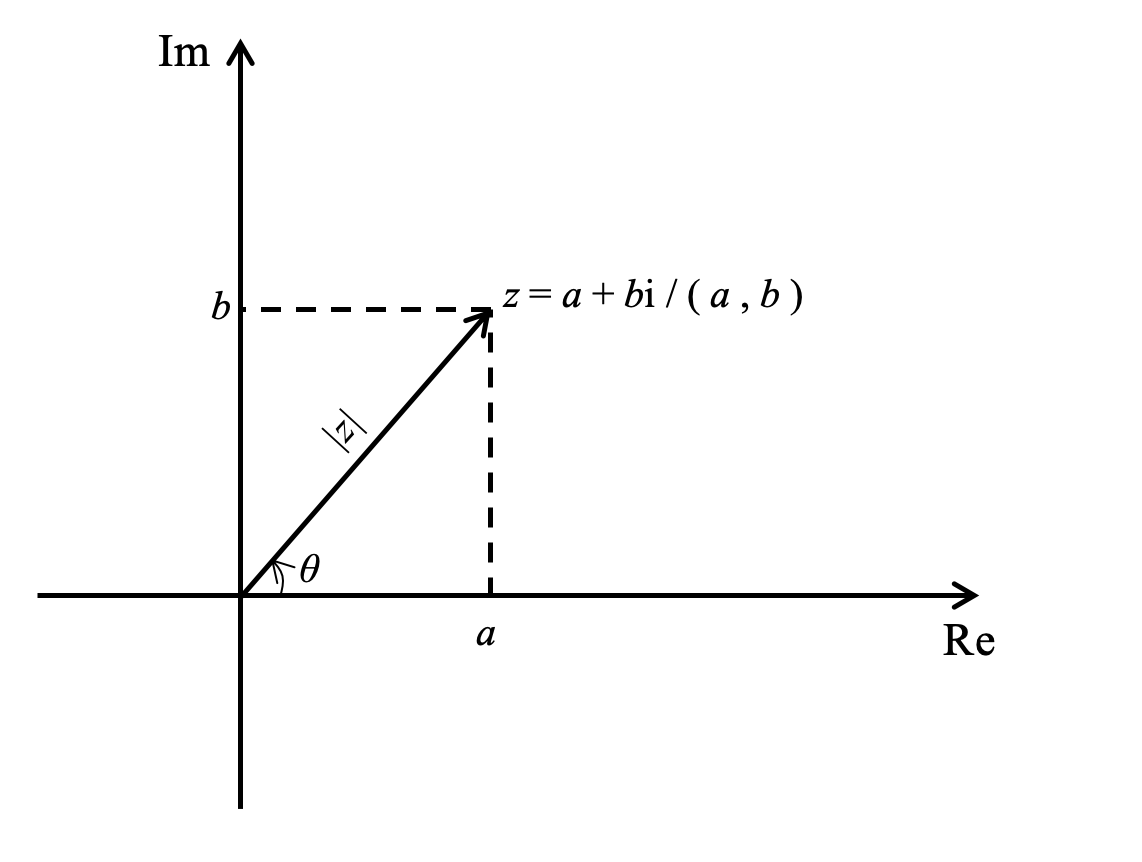
\includegraphics[width=0.5\textwidth]{Fig.1.1.jpg}
  \end{figure}
  $z=a+b\i$ can be represented on a complex plane with real coordinate $a$ and imaginary coordinate $b$. It can also be denoted as $z(a,b)$.
  \begin{itemize}
    \item Modulus of a complex number: 
    $${\color{red}{\left|z\right|=\sqrt{a^2+b^2}}}.$$
    \item Argument of a complex number: 
    $${\color{red}{\Arg(z)=\arctan\left(\frac{b}{a}\right)(+k\pi)}}{\color{green}{\ \rightarrow\ \arctan x\in\left.\right]-\frac{\pi}{2},\frac{\pi}{2}\left[\right.}}.$$
    {\color{green}{*When determine a complex number, first draw it on the plane to show which quadrant it is in.}}\\
    The range of arugment is $\left[0,2\pi\right]$ or $\left[-\pi,\pi\right]$.
    \item Use modulus and argument to express a complex number: 
    $${\color{red}{a=\left|z\right|\cdot\cos\theta}};$$
    $${\color{red}{b=\left|z\right|\cdot\sin\theta}}.$$
  \end{itemize} 
  \item If $z=a+b\i$ and $|z|=1$, then {\color{red}{$z^*=z^{-1}$}}.
  \begin{proof}{1.6.2.1}{}
    $$\begin{aligned}
      &\because |z|=1\\
      &\therefore \sqrt{a^2+b^2}=1\\
      &\therefore a^2+b^2=1
    \end{aligned}$$
    \begin{multicols}{2}
    \begin{boxed}{\text{Method 1}}\end{boxed}
    $$\begin{aligned}
      \text{RHS}=z^{-1}&=\frac{1}{a+b\i}=\frac{a-b\i}{(a+b\i)(a-b\i)}\\
      &=\frac{a-b\i}{a^2+b^2}=a-b\i\\
      &=z^*=\text{LHS}.
    \end{aligned}$$
    \begin{boxed}{\text{Method 2}}\end{boxed}
    $$\begin{aligned}
      z\cdot z^*&=(a+b\i)(a-b\i)\\
      &=a^2+b^2\\
      &=|z|^2=1\\
      \therefore \ &\ z^*=z^{-1}
    \end{aligned}$$
    \end{multicols}
  \end{proof}
  \item When $|z|\neq 1$, {\color{red}{$z^*=\frac{|z|^2}{z}$}}, and {\color{red}{$z^{-1}=\frac{z^*}{|z|^2}$}}.
  \item Properties of modulus and arguments: \\
  For complex number $s$ and $t$ $\in\C$: 
  \begin{itemize}
    \item $$|st|=|s||t|$$
    \item $$\left|\frac{s}{t}\right|=\frac{|s|}{|t|}$$
    \item $$\Arg(st)=\Arg(s)+\Arg(t)+2k\pi$$
    \item $$\Arg\left(\frac{s}{t}\right)=\Arg(s)-\Arg(t)+2k\pi$$
  \end{itemize}
\end{enumerate}

\subsection{Complex Number in Other Forms}
\begin{enumerate}
  \item The Polar Form (Modulus-Argument Form): 
  \begin{itemize}
    \item $${\color{red}{z=r(\cos\theta+\i\sin\theta)=r\cis\theta}}$$
    \begin{proof}{1.6.3.1}{}
      According to the Argand Diagram: 
      $$z=x+y\i=r\cos\theta+\i r\sin\theta=r(\cos\theta+\i\sin\theta).$$
    \end{proof}
    \item $${\color{red}{z_1z_2=r_1r_2\cis(\theta_1+\theta_2)}}$$
    \item $${\color{red}{\frac{z_1}{z_2}=\frac{r_1}{r_2}\cis(\theta_1-\theta_2)}}$$
  \end{itemize}
  \item de Movrie's Theorem: 
  \begin{itemize}
    \item By Maclaurin Series: $${\color{red}{e^{\i\theta}=\cis\theta}}=\cos\theta+\i\sin\theta.$$
    \item Exponential form of complex number: 
    $${\color{red}{z=re^{\i\theta}=r\cis\theta}}.$$
  \end{itemize}
  \item Cartesian Form: Addition and Substraction\\
  Modulus-Argument Form: Multiply and Division\\
  Exponential Form: Exponents and Roots
  \item Since $\cis\theta=\cis(\theta+2k\pi),$ 
  $${\color{red}{re^{\i\theta}=re^{\i(\theta+2k\pi)}}}.$$
  \begin{example}{1.6.3.1}{}
    \textbf{Find $e^{\i\frac{17\pi}{12}}$ in the form of Cartesian.}\\
    \noindent\rule[0.25\baselineskip]{\textwidth}{1pt}
    $$\begin{aligned}
      e^{\i\frac{17\pi}{12}}=e^{\i\left(\frac{7\pi}{6}+\frac{\pi}{4}\right)}&=e^{\i\frac{7\pi}{6}}\cdot e^{\frac{\pi}{4}}\\
      &=\cis\left(\frac{7\pi}{6}\right)\cdot\cis\left(\frac{\pi}{4}\right)\\
      &=\left(-\frac{\sqrt{3}}{2}-\frac{1}{2}\i\right)\left(\frac{\sqrt{2}}{2}+\frac{\sqrt{2}}{2}\i\right)=\frac{\sqrt{2}-\sqrt{6}}{4}-\frac{\sqrt{2}+\sqrt{6}}{4}\i.
    \end{aligned}$$
  \end{example}
\end{enumerate}

\subsection{Power of Complex Number}
\begin{enumerate}
  \item For a complex number $z=re^{\i\theta},$
  $${\color{red}{z^n=r^ne^{\i n\theta}}}.$$
  \begin{example}{1.6.4.1}{}
    \textbf{Find $\left(3\cos\frac{2\pi}{3}-3\i\sin\frac{\pi}{3}\right)^3$}\\
    \noindent\rule[0.25\baselineskip]{\textwidth}{1pt}
    $$\begin{aligned}
      \left(3\cos\frac{2\pi}{3}-3\i\sin\frac{\pi}{3}\right)^3&=\left(-3\cos\frac{\pi}{3}-3\i\sin\frac{\pi}{3}\right)^3\\
      &=\left(-3\left(\cos\frac{\pi}{3}+\i\sin\frac{\pi}{3}\right)\right)^3\\
      &=(-3)^3(e^{\i\frac{\pi}{3}})^3\\
      &=-27e^{\i\pi}\\
      &=-27(-1)=27.
    \end{aligned}$$
    {\color{green}{Key learnings from Example 6.4.1: \\
    1. $z=3$ is only the fundemental root of equation $z^3=27$. In $\C$, there are other two complex roots that satisfy the euqation.\\
    2. In $\C$, $\sqrt{4}=\pm 2=2+0\cdot\i\text{ or }-2+0\cdot\i$.}}
  \end{example}
  \begin{example}{1.6.4.2}{}
    \textbf{Given a complex number $\omega\neq 1$ is one of the solutions of $z^3=1.$\\
    a. Prove $\omega^2+\omega+1=0$;\\
    b. Calculate $\omega^{2019}+\omega^{2020}+\omega^{2021}+\omega^{2022}$.}\\
    \noindent\rule[0.25\baselineskip]{\textwidth}{1pt}
    \begin{enumerate}
      \item \begin{boxed}{\text{Approach A}}\end{boxed}
      $$\begin{aligned}
        &\because \omega^3=1\\
        &\therefore \omega^3-1=0\ \Rightarrow\ (\omega-1)(\omega^2+\omega+1)=0\\
        &\because \omega\neq 1\\
        &\therefore \omega^2+\omega+1=0.
      \end{aligned}$$
      \begin{boxed}{\text{Approach B}}\end{boxed}
      $\omega^2+\omega+1=0$ is a geometric sequence, $u_1=1,\ r=\omega:$
      $$S_3=\frac{u_1(1-r^3)}{1-r}=\frac{1-\omega^3}{1-\omega}=\frac{0}{1-\omega}=0.$$
      \item $$\begin{aligned}
        \omega^{2019}+\omega^{2020}+\omega^{2021}+\omega^{2022}&=\omega^{2019}\times(1+\omega+\omega^2+\omega^3)\\
        &=\omega^{2019}(0+1)=\omega^{2019}\\
        &=\left(\omega^{3}\right)^{673}=1.
      \end{aligned}$$
    \end{enumerate}
  \end{example}
  \begin{example}{1.6.4.3}{}
    \textbf{Find: \\
    a. $1^\i$;\\
    b. $\ln(-1)$;\\
    c. $\ln(-c)$, where $c$ is a constant. }\\
    \noindent\rule[0.25\baselineskip]{\textwidth}{1pt}
    \begin{enumerate}
      \item $$1=e^{\i 2\pi}\ \Rightarrow\ 1^\i=\left(e^{\i 2\pi}\right)^\i=e^{-2\pi}. \ \ \ \ {\color{green}{(1^\i=e^{-2k\pi}, k\in\Z)}}$$
      \item $$-1=e^{\i\pi}\ \Rightarrow\ \ln(-1)=\ln\left(e^{\i\pi}\right)=\i\pi.$$
      \item $$\ln(-c)=\ln\left[(-1)\cdot c\right]=\ln(-1)+\ln(c)=\ln(c)+\i\pi.$$
    \end{enumerate}
  \end{example}
\end{enumerate}

\subsection{Polynomial Function with Complex Roots}
\begin{enumerate}
  \item Conjugate Pair Theorem: 
  \begin{theorem}{1.6.5.1 Conjugate Pair Theorem}{}
    If $z$ is a complex root of $P(x)$, then the conjugate of $z(z^*)$ is also a complex root of $P(x)$. ($P(x)$ should be a polynomial with {\color{red}{rational}} coefficients.)
  \end{theorem}
  \item Properties of Conjugate. 
  \begin{itemize}
    \item $$(s\pm t)^*=s^*\pm t^*$$
    \item $$(st)^*=s^*t^*$$
    \item $$\left(\frac{s}{t}\right)^*=\frac{s^*}{t^*}$$
  \end{itemize}
\end{enumerate}

\subsection{Root of Complex Numbers}
\begin{enumerate}
  \item The Root of Unity: 
  \begin{theorem}{1.6.6.1 The Root of Unity}{}
    For any complex equation $\omega^n=1$, there are $n$ distinct roots: 
    $$1=e^{\i(0+2k\pi)}=\omega^n,\ k\in\Z\ \ \ \ \Rightarrow\ \ \ \ \omega=e^{\i\frac{2k\pi}{n}},\ k\in\Z.$$
  \end{theorem}
  \begin{example}{1.6.6.1}{}
    \textbf{Solve $z^3=8$.}\\
    \noindent\rule[0.25\baselineskip]{\textwidth}{1pt}
    $$\begin{aligned}
      z^3=8\cdot 1=8e^{i(0+2k\pi)}\ &\ \Rightarrow\ \ z=2e^{i\frac{2k\pi}{3}},\ k\in\Z\\
      k&=0:\ z=2\\
      k&=1:\ z=2e^{i\frac{2\pi}{3}}=2\cis\left(\frac{2\pi}{3}\right)=-1+\sqrt{3}\i\\
      k&=2:\ z=2e^{i\frac{4\pi}{3}}=2\cis\left(\frac{4\pi}{3}\right)=-1-\sqrt{3}\i
    \end{aligned}$$
  \end{example}
  \item Property of $\cis\theta$: 
  $$\cis(-\theta)=\cos\theta-\i\sin\theta$$
  \begin{proof}{1.6.6.1}{}
    $$\begin{aligned}
      \cos\theta-\i\sin\theta&=\cos(-\theta)+\i\sin(-\theta)\\
      &=\cis(-\theta).
    \end{aligned}$$
  \end{proof}
\end{enumerate}
\end{document}